\documentclass[../main.tex]{subfiles}
\begin{document}
Chapter~\ref{chapter:intro} has discussed the problems which lead to the motivations of this thesis. It has also presented the objectives, the tentative solutions, and the contributions of this thesis. There are two main parts in this chapter. They are presentations about (i) related works in Section~\ref{sec:related}, and (ii) the foundation theory in Section~\ref{sec:foundtheo}. Specifically, in Section~\ref{sec:foundtheo}, models, and algorithms contributing to the making of the lightweight module on edge devices will be introduced in detail. For the purpose and scope of the thesis, four main components that make up the proposed human monitoring module on edge devices will be introduced including: (i) object detection with YOLOv5 in Section~\ref{sec:objdect}, (ii) object tracking algorithms including SORT and DeepSORT in Section~\ref{sec:objtrack}, (iii) deep metric learning with particular emphasis on the hard triplet loss function in Section~\ref{sec:deepmetric}, and (iv) MobileNetV2 architecture in Section~\ref{sec:mbv2}.

\section{Related works}
\label{sec:related}


\subsection{Person Re-Identification}
\label{sec:personreid}



\subsection{Edge Computing in AI}
\label{sec:edgecomputing}

Edge computing has emerged as a transformative paradigm in artificial intelligence, bringing computational capabilities closer to data sources and end users. The global edge AI market size was estimated at USD 20.78 billion in 2024 and is anticipated to grow at a CAGR of 21.7\% from 2025 to 2030 \cite{grandview2024}. This rapid growth reflects the increasing demand for real-time processing, reduced latency, and enhanced privacy in AI applications.
In the context of retail and customer experience, edge computing offers significant advantages. Edge computing allows retail IT teams to optimize cloud costs by being more strategic about the data they send to the cloud, processing only the essential information instead of all the raw data \cite{biztech2024}. This selective data processing is particularly relevant for person Re-ID systems, where massive amounts of video data can be filtered and processed locally before sending relevant features to central servers.

Recent research has focused on optimizing AI models for edge deployment. Novel person Re-ID networks integrate pedestrian edge features into the representation and utilize edge information to guide global context feature extraction \cite{mdpi2024_edge}. This approach demonstrates the feasibility of running sophisticated Re-ID algorithms on resource-constrained edge devices.

The trend toward edge AI democratization is evident in various applications. Edge Intelligence or Edge AI moves AI computing from the cloud to edge devices, where data is generated, representing a key to AI democratization \cite{viso2024}. This democratization is particularly important for SMEs that cannot afford cloud-based AI solutions with high operational costs.


\subsection{Microservices and Distributed Systems}
\label{sec:microservice}

Microservices architecture has become increasingly important in developing scalable AI systems. Microservices are generally characterized by a focus on modularity, with each service designed around a specific business capability. These services are loosely coupled, independently deployable, and often developed and scaled separately \cite{wiki2024_microservices}.

In the context of person Re-ID systems, microservices offer several advantages for distributed deployment. Person Re-ID microservices over artificial intelligence Internet of Things edge computing gateways address privacy issues while enabling identification of the same person from multiple different angles across multiple cameras \cite{mdpi2021_microservice}.

The distributed nature of modern Re-ID systems presents unique challenges. Current computer vision algorithms on person Re-ID mainly focus on performance, making them unsuitable for distributed systems. For distributed systems, computational complexity becomes a critical consideration \cite{ieee2015_distributed}. This highlights the need for lightweight, distributed-friendly Re-ID algorithms that can operate efficiently across multiple edge nodes.

Recent work has explored distributed frameworks for deep learning applications. Distributed microservice deep-learning frameworks for object detection in edge computing involve analyzing images and videos to extract information about object classes and their locations \cite{mdpi2023_framework}. These frameworks provide a foundation for building scalable Re-ID systems that can handle multiple cameras and locations.

Cloud-based distributed approaches have also been investigated. Video-based person Re-ID based on distributed cloud computing uses distributed data storage methods, storing pedestrian datasets and parameters in cloud nodes with data redundancy mechanisms to increase fault tolerance \cite{jait2022_cloud}. However, such approaches may not be suitable for cost-sensitive SME deployments due to ongoing cloud costs.

The evolution toward microservices in AI applications reflects broader trends in software architecture. While there are similarities between microservices and distributed systems, microservices are an approach to design where an application is broken into multiple smaller services that can be deployed independently \cite{splunk2024}. This independence is crucial for Re-ID systems deployed across multiple retail locations, where individual components may need updates or maintenance without affecting the entire system.




\section{Foundation theory}
\label{sec:foundtheo}

\subsection{Object detection}
\label{sec:objdect}

Object detection technology finds applications across numerous domains including automatic traffic violation systems, identification of unfamiliar persons, digital attendance systems, and autonomous robotic vehicles. The advent of deep learning has dramatically enhanced object detection capabilities. Region-Based Convolutional Neural Networks (R-CNN) \cite{girshick2014richfeaturehierarchiesaccurate} represented one of the pioneering breakthroughs in this area, combining CNN architectures \cite{oshea2015introductionconvolutionalneuralnetworks} with region proposal mechanisms to achieve accurate object localization and classification in images. Subsequent iterations, Fast R-CNN \cite{girshick2015fastrcnn} and Faster R-CNN \cite{ren2016fasterrcnnrealtimeobject}, were developed to enhance both processing speed and detection precision compared to the original model. Despite these improvements in detection performance, the multi-step processing pipeline made these approaches impractical for real-time applications.

Modern frameworks such as Detectron2 \cite{Merz_2023} and EfficientDet \cite{tan2020efficientdetscalableefficientobject} have pushed object detection forward considerably. Detectron2 offers flexible deployment of high-performing models but demands extensive setup and typically involves computationally heavy architectures, making it unsuitable for real-time or resource-limited environments. EfficientDet provides a more practical option for devices with constrained resources, though it may struggle to meet strict real-time performance criteria.

You Only Look Once (YOLO) addresses the limitations of multi-stage detection approaches by reformulating object detection as a single regression problem. YOLO processes the entire image in one forward pass, directly predicting bounding boxes and class probabilities from full images. This unified architecture enables real-time performance while maintaining reasonable accuracy for many applications.

The YOLO family has evolved through multiple iterations, with each version improving upon speed-accuracy trade-offs. YOLOv11 \cite{khanam2024yolov11overviewkeyarchitectural}, in particular, offers several model variants ranging from nano (yolo11n) to extra-large (yolo11x) configurations. The nano variant is specifically designed for resource-constrained environments, featuring significantly reduced parameters and computational requirements while preserving essential detection capabilities.

\begin{figure}[h!]
\centering
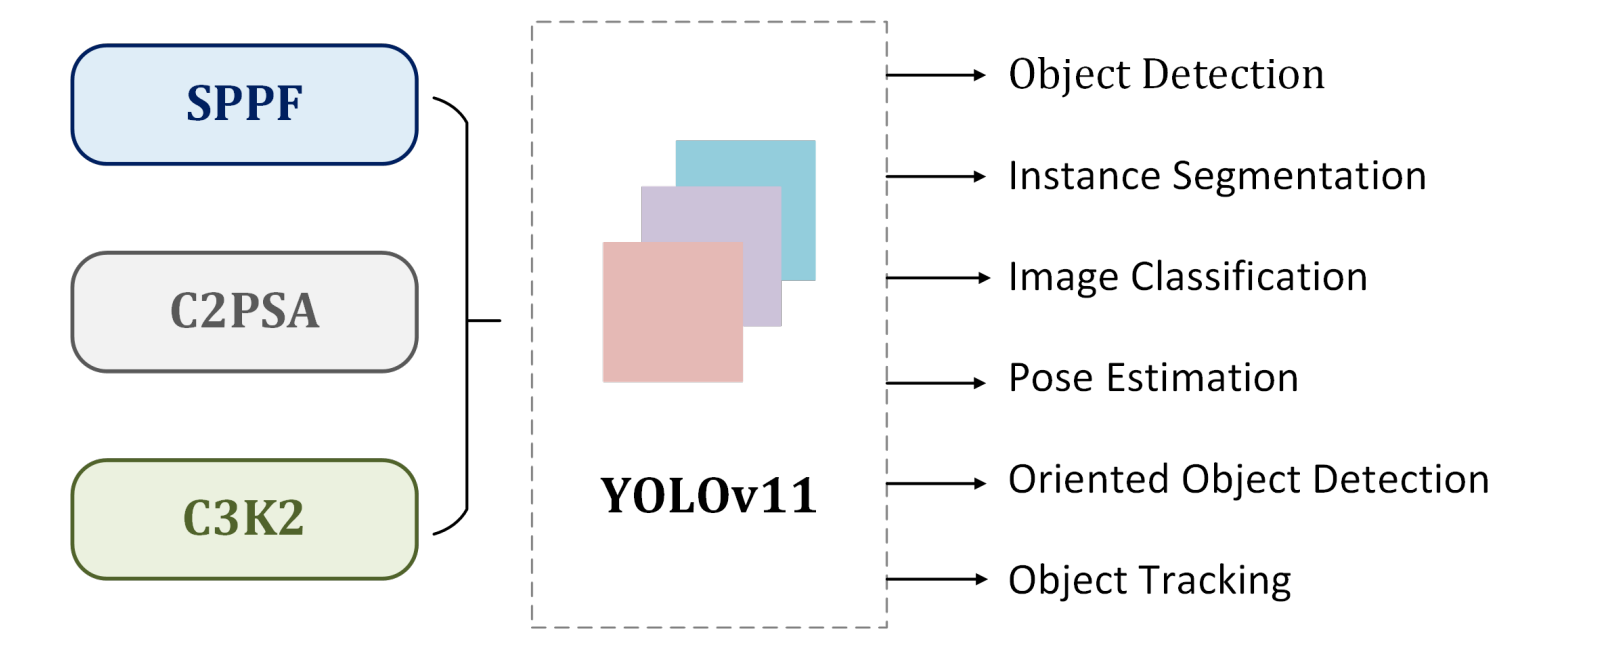
\includegraphics[width=\linewidth]{Figure/yolov11.png}
\caption{ Key architectural modules in YOLO11~\cite{khanam2024yolov11overviewkeyarchitectural}.}
\label{fig:yolov11}
\end{figure}

A significant advancement in YOLOv11 is the integration of thhe C2PSA (Convolutional
block with Parallel Spatial Attention) component, which enhances spatial attention capabilities beyond previous YOLO iterations. The C2PSA blockenables the model to focus more effectively on critical regions within images by inaplementing parallel spatial
attention mechanisms. This enhancement is particularly beneficial for detecting objects of varying sizes and positions, addressing common challengees in complex visual environments with partially occluded or small objects. The retention of the Spatial Pyramid Pooling - Fast (SPPF) blockfrom previous versions, combined with the new C2PSA component, creates a compreehensive feature processing pipeline that balances computational efficiency with enhancced spatial awareness.

For edge-based human monitoring applications, YOLOv11n provides an optimal balance between detection performance and computational efficiency. Its lightweight architecture enables deployment on edge devices for real-time person detection, serving as the foundation for subsequent tracking and Re-ID processes in distributed camera networks.

\subsection{Object tracking}
\label{sec:objtrack}

Person Re-ID systems face significant challenges when relying solely on frame-by-frame analysis. Individuals frequently lose their visual identity due to various factors including occlusions from other people or objects, rapid movement causing motion blur, and temporary disappearance from camera coverage areas. While deep learning-based feature extraction models can effectively capture contextual information and compute discriminative identity embeddings, frame-based matching approaches often suffer from identity fragmentation—where the same person receives multiple different identities across consecutive frames.

To address these limitations, tracking mechanisms play a crucial role in maintaining identity consistency over temporal sequences. Unlike existing methods that perform Re-ID independently for each frame, tracking-based approaches maintain continuous identity associations across time. This temporal continuity significantly outperforms computationally expensive alternatives such as query-driven region proposals \cite{munjal2019queryguidedendtoendpersonsearch} and graph-based retrieval methods \cite{zhu2025graphbasedapproachesfunctionalitiesretrievalaugmented}, which become prohibitively costly in large-scale deployment scenarios. By leveraging tracking, our system can efficiently associate multiple detections of the same person, substantially reducing redundant identity searches while improving real-time processing capabilities.

The development of multi-object tracking (MOT) algorithms has evolved through several generations, each addressing specific limitations of previous approaches. 

Multi-object tracking has evolved through several approaches, each with distinct trade-offs. SORT \cite{sort} provides efficient tracking by integrating object detection with motion prediction, but struggles with complex movement patterns and fast-paced scenarios. To address these limitations, DeepSORT \cite{deepsort} incorporates appearance features via a pre-trained Siamese network, improving performance in dense environments where motion alone is inadequate. However, this enhancement introduces dependency on embedding quality and computational complexity, making it susceptible to visual disturbances. FairMOT \cite{fairmot} advances this paradigm by merging detection and tracking into a unified architecture that simultaneously produces detection outputs and Re-ID features for enhanced multi-object tracking. This unified approach, while effective, demands significant computational resources and requires careful optimization between detection and Re-ID objectives, ultimately compromising processing speed. Alternative solutions include MMTracking \cite{mmtracking}, which provides a versatile framework supporting multiple advanced algorithms but necessitates substantial parameter optimization.

ByteTrack \cite{bytetrack} represents a breakthrough in tracking methodology, delivering exceptional performance without requiring dedicated appearance models, thereby maintaining high processing speeds particularly in crowded environments. This approach achieves an optimal trade-off between real-time processing and tracking reliability. Consequently, our framework employs ByteTrack for maintaining pedestrian identity consistency across video frames, significantly enhancing ID assignment precision. This capability proves essential in dense scenarios where overlapping persons create significant challenges for camera-based identification systems.

\subsection{Feature extraction}
\label{sec:feature_extraction}

Feature extraction serves as the cornerstone of person Re-ID systems, converting raw image data into discriminative descriptors that enable robust identity matching. Various research efforts have focused on enhancing feature extraction efficiency, particularly for deployment on resource-constrained edge devices.

Several approaches have explored image preprocessing techniques to enhance feature extraction quality under challenging conditions. Yan et al. \cite{app12157825} proposed a weighted object detection framework that selectively emphasizes salient image regions to generate more discriminative global representations. Building upon this work, Yan et al. \cite{yan2021hybrid} developed a hybrid neural network architecture incorporating specialized preprocessing modules, demonstrating robust performance under varying illumination conditions and pose variations. Further extending these preprocessing strategies, Yan et al. \cite{yan2022gan} investigated Generative Adversarial Network (GAN)-based image enhancement techniques as preprocessing steps, effectively addressing common surveillance challenges such as poor lighting conditions and low-resolution imagery that typically compromise Re-ID performance.

While these preprocessing approaches demonstrate effectiveness in improving feature quality, they present significant limitations for edge-based deployment scenarios. The additional computational overhead and memory requirements introduced by these techniques exceed the processing capabilities of typical edge hardware. GAN-based enhancement methods, in particular, demand substantial computational resources that are incompatible with edge device constraints. Furthermore, the increased processing latency introduced by these preprocessing stages renders them unsuitable for real-time applications requiring immediate response.

Contemporary research has also explored Transformer-based architectures for enhanced feature extraction, particularly Vision Transformers (ViT) \cite{dosovitskiy2021imageworth16x16words}, which leverage self-attention mechanisms to capture long-range spatial dependencies within images. Despite their demonstrated effectiveness, these models typically require substantial computational resources, making them challenging to deploy on edge devices without extensive optimization. Multi-scale feature extraction approaches, exemplified by Feature Pyramid Networks (FPN) \cite{lin2017featurepyramidnetworksobject}, have shown promise in capturing both low-level and high-level semantic information. This approach proves particularly beneficial for Re-ID scenarios involving significant variations in object scale and camera distance. However, when implemented with large backbone networks, these methods remain computationally prohibitive for edge deployment.

To address these computational constraints, our research emphasizes lightweight feature extraction methodologies. Mobile-optimized architectures such as MobileNetV2 \cite{sandler2019mobilenetv2invertedresidualslinear} and MobileNetV3 \cite{howard2019searchingmobilenetv3} have gained prominence in edge-based applications due to their depth-wise separable convolutions that significantly reduce computational complexity while maintaining competitive accuracy. Squeeze-and-Excitation Networks (SE-Net) \cite{hu2019squeezeandexcitationnetworks} further enhance CNN architectures by implementing adaptive channel-wise feature recalibration, enabling models to focus on the most informative image regions without substantially increasing model complexity.

However, these generic lightweight models lack specific optimization for person Re-ID tasks. This limitation has motivated the development of specialized lightweight architectures tailored specifically for Re-ID applications.

OSNet (Omni-Scale Network) \cite{zhou2019omniscalefeaturelearningperson} represents a significant advancement in lightweight Re-ID architectures. OSNet uses only 2.2 million parameters, substantially fewer than traditional ResNet-50-based approaches which employ 24 million parameters, making it particularly suitable for edge deployment. OSNet introduces innovative omni-scale feature learning that captures multi-scale information through a novel building block design, enabling effective feature extraction across different spatial scales without the computational overhead of traditional multi-scale approaches. The architecture employs depth-wise separable convolutions and efficient channel shuffling operations to maintain computational efficiency while preserving discriminative capability.

LightMBN (Lightweight Multi-Branch Network) \cite{Herzog_2021} further advances edge-optimized Re-ID by introducing a multi-branch architecture specifically designed for resource-constrained environments. LightMBN incorporates efficient attention mechanisms and feature fusion strategies that maximize discriminative power while minimizing computational requirements. The network architecture employs channel-wise and spatial attention modules that adaptively emphasize important features without introducing significant computational overhead.

Despite these advances, current lightweight models still face challenges in balancing computational efficiency with discriminative capability, particularly in scenarios involving significant pose variations, occlusions, and lighting changes. Our research addresses these limitations by investigating custom-trained lightweight architectures that are specifically optimized for the unique requirements of SME deployment scenarios, emphasizing both computational efficiency and robust performance across diverse operational conditions.


\subsection{Message queue}
\label{sec:message_queue}

\subsection{Containerization}
\label{sec:containerization}

\subsection{Vector database}
\label{sec:vector_database}

\end{document}